\newpage
\section{Introduction}

\section{Clathrates, nucleation and growth}

Clathrate hydrates are cristalline inclusion compounds in which water molecules form, via hydrogen bonding, a network of polyhedral cages trapping guest molecules. Put simply, clathrates can be seen as another form of solid water. An ``empty'' clathrate cannot exist, the stability of a clathrate is guaranteed by the presence of the guest molecule. They were discovered in 1810 by Humphry Davy, and were considered only as laboratory curiosities at first. But then, Hammerschmidt discovered in 1934 that clathrates hydrates can form inside oil and gas pipelines, creating a plug that could damage the equipment, or at least reduce the flow. That is the reason why researches about them were getting more and more active since the 1950's.

Among the multiple applications of clathrates one can note:
\begin{itemize}
    \item Storage and transport of natural gases or dihydrogen. The latter option is very interesting since the storage of dihydrogen is hard at the moment
    \item A way of reducing cooling systems energy consumption and environmental impact
\end{itemize}

There are signs of great natural reserves of methane in clathrates, formed without human action. These kind of reserve can be found in the permafrost and the ocean floor. These estimated reserves are way beyond every other fossile energy combined, and are related to the formation and dissociation of these structures.

My work is about methane hydrates, mainly their formation and growth.

Some information about nucleation:
\begin{enumerate}
    \item The nucleation of clathrates is a stochastic process and is really hard to predict. This aspect gets in the way of the comprehension of the mechanisms behind nucleation. This aspect comes from the fact that the formation of the structure requires a very precise molecular configuration
    \item The nucleation can be homogenous or heterogenous and happens usually at an interface (fluid + solid, gas + liquid, liquid + liquid). In case of a heterogenous nucleation, the energy needed to move from a state to clathrate is lessened.
    \item Hydrate seem to have a ``memory effect'' which causes a quick re-formation of the hydrate if it is not given the time to completely melt or if heated close to the dissociation temperature
\end{enumerate}
After the nucleation comes the growth, where mass and heat transfer become of major importance. However, the nucleation parameters are still important during the growth.

The question of growth and nucleation at a molecular level is a scientific challenge for mainly 2 reasons:
\begin{enumerate}
    \item The stochastic nature of this phenomenon
    \item It is hard to perform an experimental study at small time and space scales, at which hydrates form
\end{enumerate}
That is where computer simulations arrive, and more specifically molecular dynamics, even if they tend to stray away from the experimental conditions of clathrates formation, they are still a powerful tool to learn more about clathrates.


\section{Algorithms}

\subsection{About Molecular Dynamics}

Molecular Dynamics Simulation can be compared to a real experiment:

\setlength{\columnseprule}{0.4pt}
\setlength{\columnsep}{1cm}
\begin{multicols}{2}
    Experiment
    
    \begin{enumerate}
        \item We prepare a sample of the material that we wish to study
        \item We connect this sample to a measuring instrument and we measure the property of interest during a certain time interval\\
          The longer we average, the more accurate our measurement becomes
    \end{enumerate}
    \columnbreak

    Simulation
    
    \begin{enumerate}
        \item We select a model system consisting of $N$ particles and we solve \textsc{Newton}'s equations of motion for this system until the properties of the system no longer change with time (we equilibrate the system)
        \item After equilibration, we perform the actual measurement
    \end{enumerate}
\end{multicols}
In order to make a simulation in molecular dynamics, we have to express the observable quantity as a function of the position and momentum.

We will consider a simple program:
\begin{enumerate}
    \item Initialize the system (initial position and velocities) in function of the thermodynamic conditions wanted
    \item Compute the force on all particles, that means taking into account all the neighboring particles (longest part)
    \item Integrate \textsc{Newton}'s equations of motion
    \item Increase the time by the timestep $\Delta t$
    \item Compute and print the average of measured quantities and stop
\end{enumerate}
This algorithm applies for a simple atomic system. In this algorithm, the longest part is the calculation of the force acting on the particles. However, time is not an issue, it must indeed be taken into account, but there is more. Computations in molecular dynamics take a really long time, and need a lot of integration steps to reach thermodynamic equilibrium, especially when dealing with growth processes. Therefore it is better to have an algorithm as accurate as possible than a fast one in order to minimize the error on the molecular interaction energy computation.

When talking about simulation, one can think of the Monte Carlo method, which is a non-time dependant simulation consisting of a random sample taken from a population and statistical analysis of the results. However, this method will not work in this kind of study. We are interested in the trajectory of the particles throughout the simulation, the growth process is dynamic and is function of the time, therefore molecular dynamics simulations are more appropriate.

\subsection{Numerical methodology}
All the molecular dynamics simulations done in this project are made with the program GROMACS\footnote{GROningen MAchine for Chemical Simulations}

This study will use a system composed of 3 phases. The methane gas phase, the hydrate phase and the liquid phase with the following compositions:

\begin{itemize}
    \item methane gas phase: 160 methane molecules
    \item hydrate phase: 184 water molecules and 44 methane molecules
    \item liquid phase:
        \subitem one slab of 736 water molecules
        \subitem one slab of 736 water molecules and 128 methane molecules (supersaturated water slab)
\end{itemize}

The dynamic simulation of the system is done in multiple steps:

The first step is a minimization of the energy of the system. After that, an equilibration (relaxation) is done at a temperature of \SI{200}{\kelvin} and a pressure of \SI{30}{\mega\pascal} for \SI{20}{\pico\second}. Once the system is equilibrated, we heat it (annealing) at a rate of \SI{0.5}{\kelvin\per\pico\second}. After the annealing, the system is in conditions to observe clathrate growth. The next step is then an NPT simulation for \SI{40}{\nano\second} at \SI{30}{\mega\pascal} to obtain the growth of clathrates.

Once this simulation is done, we can start the study on the melt of the clathrates. For that we start another batch of simulations. For all the following simulations, the starting system will be taken just after the NPT simulation at \SI{260}{\kelvin}. The melt is done in two steps: firstly we heat the system to the desired temperature, then we once again do an NPT simulation at the desired temperature, this time for \SI{20}{\nano\second}. These melt simulations will be done for several barostats: 10, 30, 60 and \SI{100}{\mega\pascal}. For each barostat, the system will be heated to 270, 280, 290 and \SI{300}{\kelvin}.

The main objectives here are to find the equilibrium point of the clathrate at different pressures, the temperature at which this equilibrium is broken (called melting point), find the distribution of cages (small, large, interface and irregular) at different point of the simulation.

\subsection{Analysis algorithm}
There are 3 methods that we will use to sort and identify the different structures. The number of water molecule in the neighbourhood of a methane molecule, the AOP of each water molecule in this neighbourhood and the hydrogen bonds between these molecules.

The first step in the analysis is to search for neighbouring water molecules for every methane molecule. In practice, the search is made between the carbon atom of the considered molecule and the neighbouring oxygen atoms.
Any oxygen atom located in a radius of \SI{5.5}{\angstrom} of the atom of interest is considered a neighbour. The number of neighbours for each methane molecule is noted $n_w$.

Among these molecules, we once again search for neighbours, this time the center molecule is a water molecule and we search for neighbouring water molecules in a radius of \SI{3.5}{\angstrom}.
These neighbours are used to compute an index called the Angular Order Parameter (AOP). This index gives us information concerning the structure of a water molecule.
\[
    \text{AOP} = \sum \left( \left( \left|\cos \theta \right| \cos \theta \right) + \cos^2 (109.47)\right)^2
\]
where $\theta$ is the angle between any pair of oxygen atoms in the neighbouring of the atom of interest (taken as the elbow of the angle). For example if an oxygen has 4 atoms in its neighbourhood, there are 6 angles to consider. The value of the AOP indicates the structure the considered water molecule belongs to:

\begin{itemize}
    \item AOP = \num{0}: ice
    \item AOP = \num{0.1}: hydrate cristaline structure
    \item AOP = \num{0.8}: liquid water (amorphous)
\end{itemize}

These values are averages, and for this study we will only consider molecules with an AOP < \num{0.4}, considered hydrate-like molecules. The number of hydrate-like molecules among the neighbours is noted $n_h$.

The last point to consider is the hydrogen bonding between the water molecules. Since the oxygen has a high electronegativity, there is a high chance of hydrogen bonding with other water molecules if certain conditions are met. These conditions are the following:

\begin{itemize}
    \item $\SI{2.5}{\angstrom} < d_{\ce{O}^1\ce{O}^2} < \SI{3.5}{\angstrom}$ with $d_{\ce{O}^1\ce{O}^2}$ the distance between the 2 oxygen atoms 
    \item looking at the molecule with the potential donor hydrogens, we take the hydrogen the closer to both oxygen atoms (distance $\ce{O}^1-\ce{H}-\ce{O}^2$), the angle $\widehat{\ce{O}^1\ce{H}\ce{O}^2}$ must be between \SI{90}{\degree} and \SI{180}{\degree}
\end{itemize}
If these 2 conditions are met, the hydrogen is considered a donor atom and a hydrogen bond is counted between the 2 molecules. The number of hydrogen bonds among the hydrate-like molecules in the neighbourhood of a methane molecule is noted $n_b$.

After the computation of these 3 numbers, we can recognise clathrates. If $n_w = n_h = 24$ and $n_b = 36$, the methane is imprisonned in a large cage; if $n_w = n_h = 20$ and $n_b = 30$, the methane is imprisonned in a small cage; if $10 < n_h < 13$, the methane is in a half-complete cage (interface cage); if $n_h \leq 14$ and $n_h \neq 20, 24$, the methane is in an irregular cage; if anything else, the methane is not considered in a cage.

A point of interest is the width of the clathrate phase throughout the melt simulation. Once we know which molecule is/is not in a cage, it is rather easy to find the width of the clathrate phase. We take the carbon atoms in large and small cages and compute the difference between the lowest and the highest values of $x$. That gives us a rough idea of the width of the clathrate phase for the frame. Doing this for several frame of the same simulation shows us if the phase if reducing or not and therefore, if the clathrates are melting.

\newpage
\section{Results and discussion}

\subsection{Growth}
The first part of this study is about the growth of clathrates at \SI{30}{\mega\pascal} and \SI{260}{\kelvin}. What follows are 3 snapshots taken at the beginning, halfway through and at the end of the simulation.

\begin{figure}[htbp]
    \centering
    \begin{subfigure}[b]{1.\linewidth}
        \centering
        \includegraphics[width=.99\linewidth]{figures/growth-frame1.png}
        \caption{Snapshot at $t = \SI{0}{\nano\second}$}
        \label{fig:snap1-prod}
    \end{subfigure}
    \begin{subfigure}[b]{1.\linewidth}
        \centering
        \includegraphics[width=.99\linewidth]{figures/growth-frame2001.png}
        \caption{Snapshot at $t = \SI{20}{\nano\second}$}
        \label{fig:snap2-prod}
    \end{subfigure}
    \begin{subfigure}[b]{1.\linewidth}
        \centering
        \includegraphics[width=.99\linewidth]{figures/growth-frame4001.png}
        \caption{Snapshot at $t = \SI{40}{\nano\second}$}
        \label{fig:snap3-prod}
    \end{subfigure}
    \caption{Snapshots at different times of the simulation}
    \label{fig:snaps-prod}
\end{figure}

On the \autoref{fig:snap1-prod}, compared to \autoref{fig:snap-equil}, we can see a bit of a clathrate shape at the middle, it is because when the heating was approaching \SI{260}{\kelvin}, the system was almost at the conditions required for the formation of clathrate, therefore cages already started forming at that point.

On \autoref{fig:snap2-prod} and \autoref{fig:snap3-prod}, we notice that as the clathrate phase widens, the gas of methane to the right of the figures is slowly decreasing. 
The following figure shows the width of the clathrate phase during the growth process:
\begin{figure}[htbp]
    \centering
    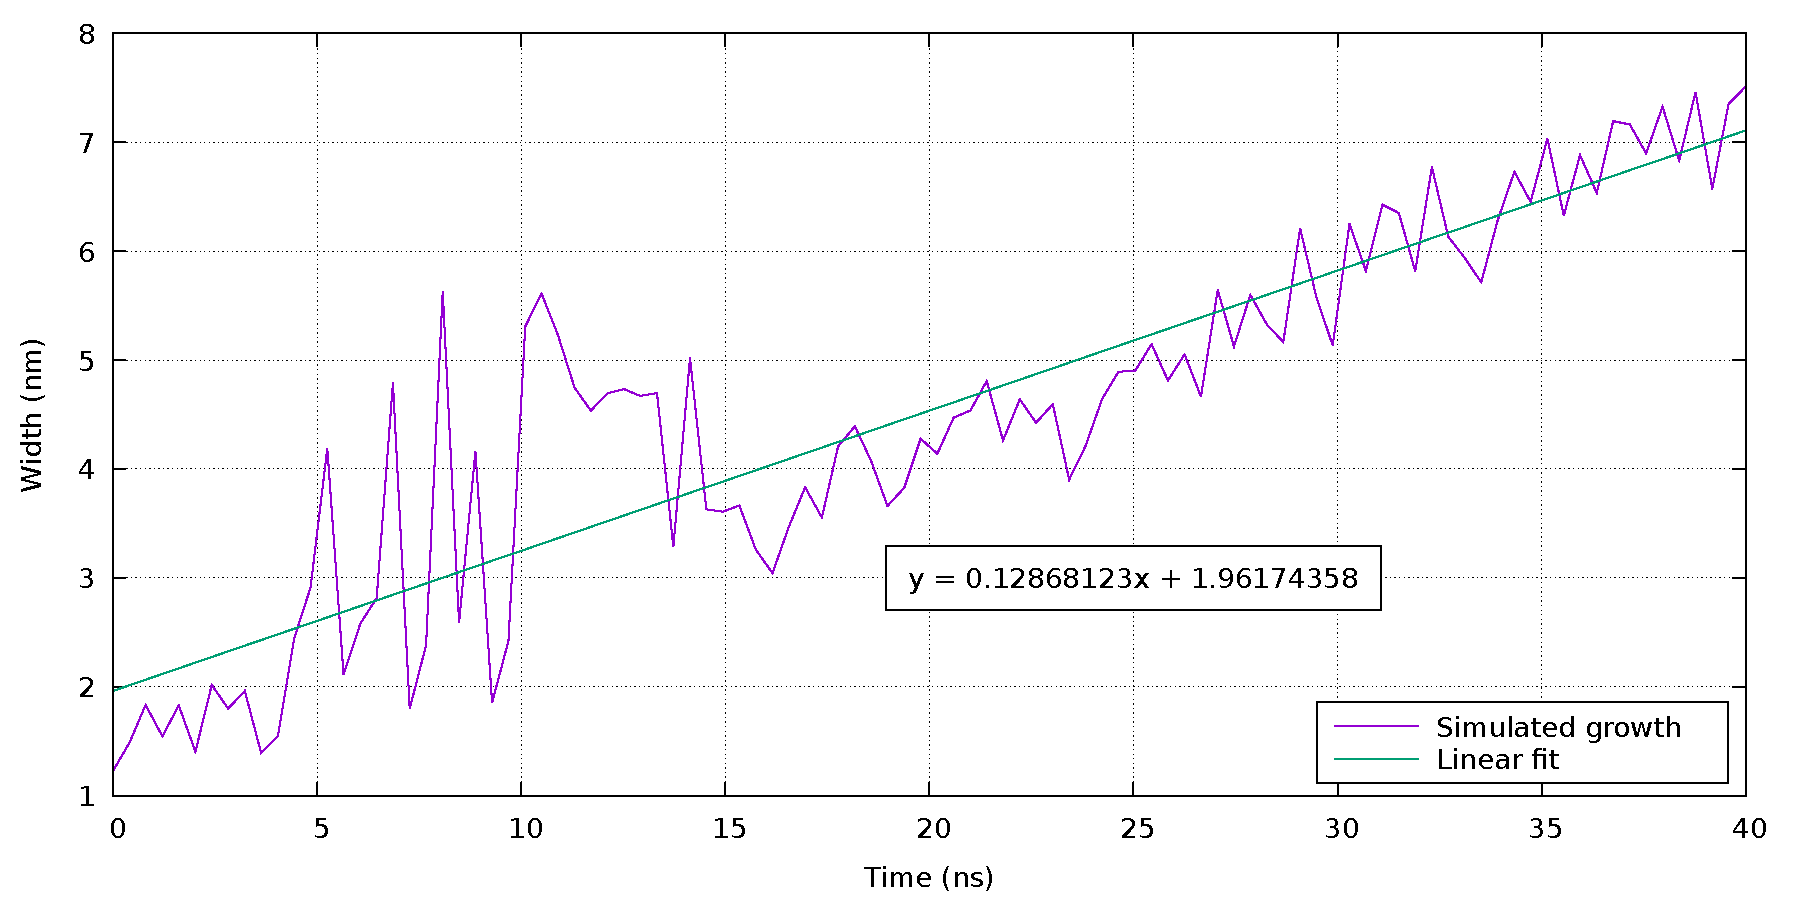
\includegraphics[width=.99\linewidth]{figures/growth-width.pdf}
    \caption{Width of the clathrate phase during growth process}
    \label{fig:width-grows}
\end{figure}

\subsection{Melt}
The second part of this study concerns the melt of the clathrates. Unlike the growth of the clathrates, the melting simulation was done at different pressures: 10, 30, 60 and \SI{100}{\mega\pascal}. The following table shows the results for the melting simulations.

\begin{table}[htbp]
    \centering
    \begin{tabular}{
        @{}
        S[table-format=3]
        S[table-format=2]
        S
        S[table-format=1.3]
        @{}
        }
        \toprule
        {Pressure} & {Simulation time} & {Melting temperature} & {Melting rate}\\
        {(\si{\mega\pascal})} & {(\si{\nano\second})} & {(\si{\kelvin})} & {(\si{\angstrom\per\nano\second})}\\
        \midrule
         10 & 20 & 295 \pm 10 & 0.130\\
         30 & 20 & 295 \pm 10 & 0.081\\
         60 & 20 & 305 \pm 10 & 0.265\\
        100 & 20 & 305 \pm 10 & 0.159\\
        \bottomrule
    \end{tabular}
    \caption{Conditions and results for the melt of clathrates}
    \label{tab:melting}
\end{table}
This first thing we notice is that for a higher pressure, the temperature needed for the clathrate to melt is higher aswell. It was expected since as predicted by thermodynamics, an increase in pressure without volume change induces a higher temperature to reach melting point.
\section{Conclusion}

\newpage
\nocite{*}
\begin{multicols}{2}
    [\center{\printbibheading}]
    \printbibliography[heading=none]
\end{multicols}

\newpage
\section{Appendices}
\begin{itemize}
    \item \textit{Description of the means used for the analysis program (docs)}
    \item \textit{Some more snapshots from the simulations (maybe)}
\end{itemize}
